\section{Word2Vec} \label{sec:Word2Vec}

% \subsection{Word Embedding Representations: Count-Based vs. Context-Based} \label{sec:CountVsContextModels}
 
%Word embeddings can be learned using two kinds of contextual vector space models: the \textbf{count-based} or \textbf{context-based vector space models}. 

%\textbf{Count-based vector space models} are unsupervised learning algorithms based on matrix factorization of a global word co-occurrence matrix. The main assumption is words in similar contexts share related semantic meanings. Examples include PCA and neural probabilistic language models. Another term for this type is \textbf{distributed semantic model} (DSM) (Weng, 2017). 

%\textbf{Context-based vector space models} are supervised algorithms that use a local context to predict target words. These are predictive models which take dense word vectors as parameters and update word representations during training.

%In 2014, Baroni et al. showed that predictive approaches outperformed count models significantly and consistently. 

%Although \textbf{Word2Vec} and \nameref{sec:Glove} are predictive and context-based vector space models, they still rely on co-occurrence counts. 

\subsection{Motivation for Word2Vec}

\textbf{Word2Vec} is an unsupervised learning algorithm for obtaining word vector representations using a two-layer neural network. Existing word representations already capture linguistic patterns, allowing algebraic operations to be done on the word vectors in their semantic vector space. But Mikolov et al. (2013b) created \textbf{Word2Vec} to learn \emph{efficient} representations from \emph{large} data, as opposed to previous architectures that reduced quality of learned vectors by using smaller data and dimensionality. 


Both the \nameref{sec:SkipGram} and \nameref{sec:CBOW} in Word2Vec are \hyperref[sec:NeuralLM]{neural network language models} with one hidden layer.  Their input vector $\overrightarrow{x} = (x_1,..., x_V)$ and output vector $\overrightarrow{y} = (y_1,...,y_V)$ are both \textbf{\hyperref[sec:OneHotEncodings]{one-hot encodings}}, and the hidden layer of the \hyperref[sec:NeuralLM]{neural network} is a \hyperref[sec:WordEmbeddings]{word embedding} with dimension $N$. 

\subsubsection{Key Concept: One-Hot Encodings} \label{sec:OneHotEncodings}

A \textbf{one-hot vector encoding} is the simplest type of word embedding where each cell in the vector corresponds to a distinct vocabulary word. A $1$ is placed in the cell marking the position of the word in the vocabulary, and $0$ elsewhere. A problem with these is they lead to high-dimensional vectors for large vocabularies, raising computational costs. Secondly, they do not let similarity between words to be represented. 

%(Thus even though the vocabulary size is $V$, the goal is to learn embeddings with size $N$). 
%For time $t$, Word2Vec predicts one output word $w_{t+j}$ (vector $\overrightarrow{y}$) given one input word $w_t$ (vector $\overrightarrow{x}$). For \textbf{Skip-Gram}, $w_{t+j}$ is the predicted context word and $w_t$ is the input target word, but for \textbf{CBOW} $w_{t+j}$ is the predicted target word and $w_t$ is the input context word.   

%Vectors $v_w$ and $v'_w$ are two representations of word $w$. Vector $v_w$ comes from the rows of the \textit{input layer $\rightarrow$ hidden layer weight matrix} $W$, and vector $v'_w$ comes from the rows of the \textit{hidden layer $\rightarrow$ output layer weight matrix} $W'$. We call $v_w$ the \textbf{input vector} and $v'_w$ is the \textbf{output vector} of the word $w$. 


\subsubsection{Skip-Gram} \label{sec:SkipGram}

The Skip-Gram model predicts context words given a single target word. It uses a fixed sliding window to capture bidirectional context along a sentence, around a single target word. The target is input as a one-hot encoding to a neural network which updates the target vector with values near $1$ in cells corresponding to predicted context words (Weng, 2017).  The Skip-Gram is illustrated in \cref{fig:SkipGram}.

Consider the following sentence from Weng (2017): ``The man who passes the sentence should swing the sword." Using context window size $c = 5$ and target word ``swing", the Skip-Gram should learn to predict the context words $\{$\texttt{"sentence"}, \texttt{"should"}, \texttt{"the"}, \texttt{"sword"} $\}$, and so the target-context word pairs fed into the model for training are: (\texttt{"swing"}, \texttt{"sentence"}), (\texttt{"swing"}, \texttt{"should"}), (\texttt{"swing"}, \texttt{"the"}), and (\texttt{"swing"}, \texttt{"sword"}).  



\begin{figure}
\centering
\begin{minipage}{.48\textwidth}
  \centering
  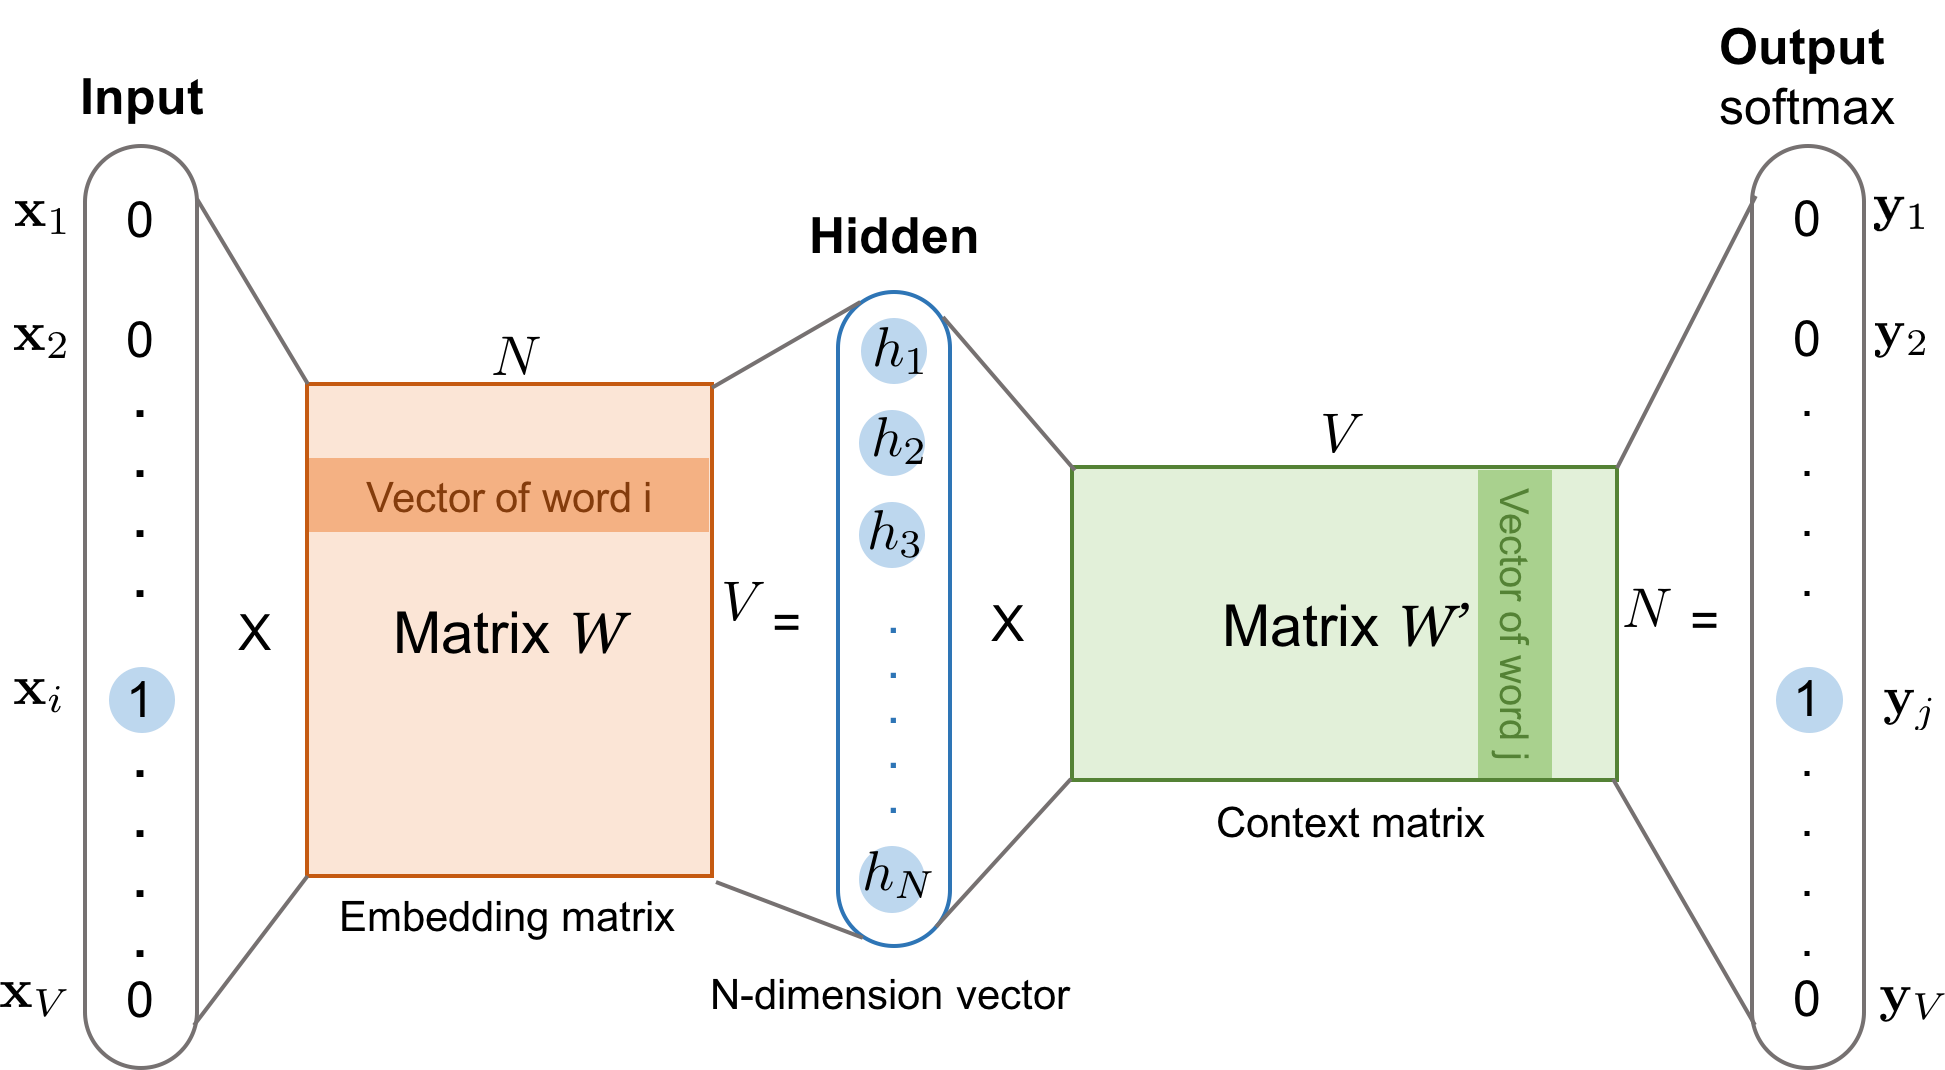
\includegraphics[width=\textwidth]{imgs/skipgram_image.png}
  \captionof{figure}{Simplified Skip-Gram Model with one input target word and one output context word. From \emph{Learning Word Embeddings}, by Lilian Weng, 2017. \url{https://lilianweng.github.io/lil-log/2017/10/15/learning-word-embedding.html}. Copyright 2017 by Weng.}
  \label{fig:SkipGram}
\end{minipage} \hspace{1.5em}%
\begin{minipage}{.48\textwidth}
  \centering
  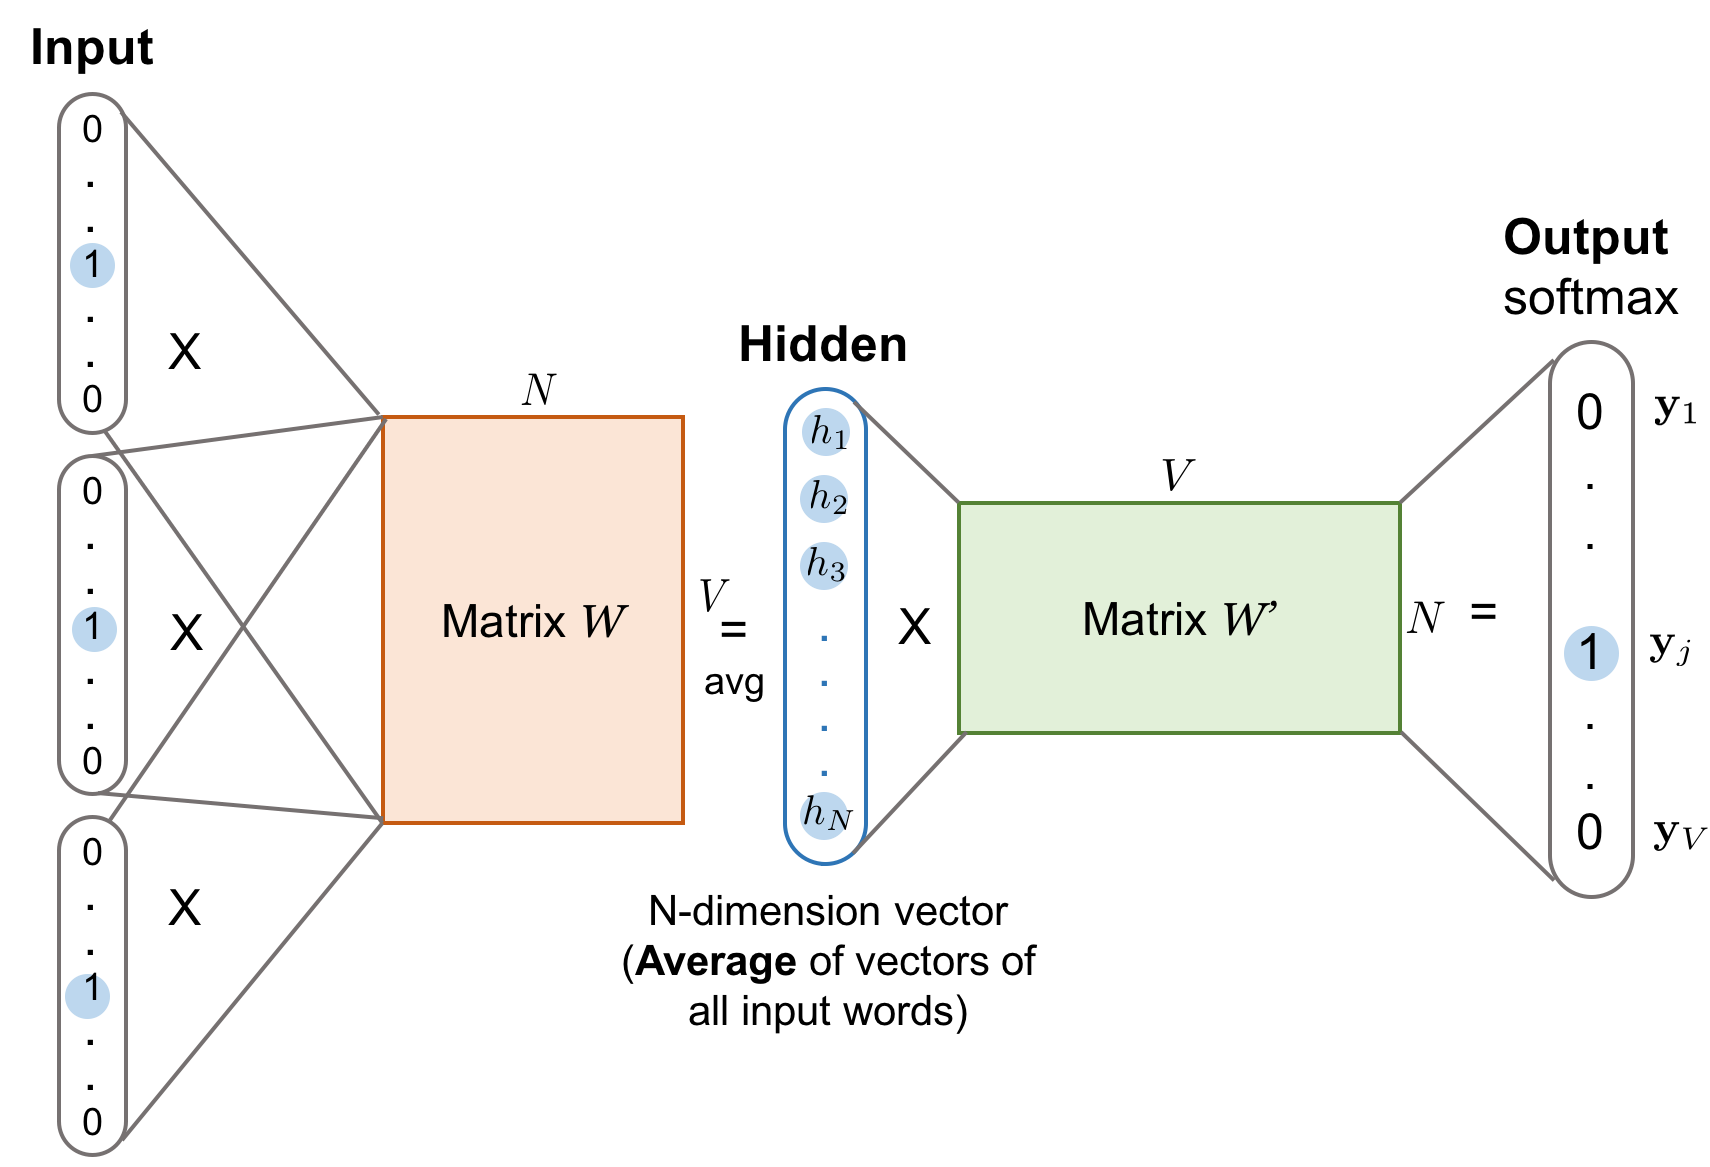
\includegraphics[width=\textwidth]{imgs/cbow.png}
  \captionof{figure}{CBOW Model with several one-hot encoded context words at the input layer and one target word at the output layer. From \emph{Learning Word Embeddings}, by Lilian Weng, 2017. \url{https://lilianweng.github.io/lil-log/2017/10/15/learning-word-embedding.html}. Copyright 2017 by Weng.}
  \label{fig:CBOW}
\end{minipage}
\end{figure}


% 
% \subsubsection{Forward and Backward Pass for Skip-Gram}
% 
% According to the Skip-Gram illustrated in \cref{fig:SkipGram}, the procedure for learning word vectors is: 
% \begin{enumerateSpaced}{3pt}
%     \item the input word $w_i$ and output word $w_j$ are encoded as one-hot vectors, $\overrightarrow{x}$ and $\overrightarrow{y}$ respectively. (For Skip-Gram, $\overrightarrow{x}$ is the target vector and $\overrightarrow{y}$ is the context vector). 
%     
%     \item A randomly initialized word embedding matrix $W$ with size $V \times N$ at the input $\rightarrow$ hidden layer is multiplied with $\overrightarrow{x}$ to give the $N$-dimensional embedding for target word $w_i$. This embedding resides in the $i$-th row of $W$ and is considered as the hidden layer of the model. 
%     
%     \item Next, the hidden layer is multiplied by weight matrix $W'$ with size $N \times V$ to produce the one-hot encoded output vector, $\overrightarrow{y}$. \textbf{NOTE: }the output context matrix $W'$ encodes words as context and is distinct from the embedding matrix $W$. 
%     
%     \item The result of the above multiplication is sent through the softmax layer to create a probability distribution over the words. The above steps constitute the \hyperref[sec:ForwardProp]{forward pass}.
%     
%     \item \hyperref[sec:ErrorCalc]{Errors} are obtained by subtracting the output vector with the target vector. 
%     
%     \item The error vector is \hyperref[sec:BackwardProp]{backward-propagated} through the neural network to update the weight matrix. The procedure continues until errors are small enough. 
%     
% \end{enumerateSpaced}
% 




\subsubsection{Continuous Bag of Words Model (CBOW)} \label{sec:CBOW}

The \textbf{continuous bag of words model (CBOW)} is opposite to Skip-Gram since it predicts the \emph{target} word based on a \emph{context} word. Generally during training, CBOW receives a window of $n$ context words around the target word $w_t$ at each time step $t$ to predict the target word (Mikolov et al., 2013b). The forward pass for CBOW is similar to Skip-Gram's, except CBOW averages context word vectors while multiplying INPUT $\overrightarrow{x}$ and the \emph{input} $\rightarrow$ \emph{hidden layer} matrix $W$. From Rong (2016), $\overrightarrow{h} = \frac{1}{c} W \cdot \Big(\overrightarrow{x_1} + \overrightarrow{x_2} + ... + \overrightarrow{x_c} \Big) = \frac{1}{c} \cdot \Big(\overrightarrow{v_{w_1}} + \overrightarrow{v_{w_2}} + ... + \overrightarrow{v_{w_c}} \Big)$, where $c$ is the number of context words, $w_1,...,w_c$ are the context words, and $v_w$ is the input vector for general word $w$. According to Weng (2016), the fact that CBOW averages distributional information of the context vectors makes CBOW better suited for small datasets. The CBOW is shown in \cref{fig:CBOW}.


\subsection{Phrase-Learning in Word2Vec Using Skip-Gram}

The problem with previous word vectors is their lack of phrase representation. ``Canada" and ``Air" could not be recognized as part of a larger concept and be combined into ``Air Canada". Many phrases have meaning that is not just a composition of the meanings of its individual words and should be represented as a unique identity. In contrast, a bigram like ``this is" should remain unchanged (Mikolov et al., 2013a, p. 5). 

As an attempt to solve this, the \textbf{Phrase Skip-Gram} forms phrases based on the score $S_{phrase} = \frac{C(w_i w_j) - \delta} {C(w_i)C(w_j)}$, where $C(\cdot)$ is the count of a unigram $w_i$ or bigram $w_i w_j$ and $\delta$ is a discounting threshold to avoid creating infrequent words and phrases. High values of $S_{phrase}$ means the phrase is most likely a phrase rather than simple concatenation of two words. Mikolov et al. (2013a) found that this Phrase Skip-Gram with hierarchical softmax and subsampling outperformed the original model on large data. 

Also, the Phrase Skip-Gram creates vectors exhibiting a linear structure called \textbf{additive compositionality}, which allows words to be combined meaningfully by adding their word vectors. Since learned context vectors can represent the overall distribution of context words in which the target word appears, and since the vectors in the loss function are logarithmically related to the probabilities from the output layer, the sum of two word vectors is related to the product of the context distributions (using the logarithm sum rule). This product of distributions acts like an AND function since words are weighted by probability. Consequently, if the key phrase ``Volga River" appears many times in the same sentence along with ``Russian" and ``river", the sum $vector(\texttt{"Russian"}) \! + \! vector(\texttt{"river"})$ results in the phrase $vector(\texttt{"Volga River"})$ or at least a vector close to it (Mikolov et al., 2013a). 
